% TeX лр6
% Автор: Балакин В.В.
% Версия от: последнего изменения декабря 2020 года.
% Сборка документа из командной строки:
\documentclass[a4paper,14pt]{extarticle}
%\usepackage[a4paper,margin=1cm,landscape]{geometry}
\usepackage[utf8]{inputenc}
\usepackage[T2A]{fontenc}
\usepackage[english,russian]{babel}

% Пакет отвечающий за рисование графиков в нутри TeX файла.
% https://ru.sharelatex.com/blog/2013/08/27/tikz-series-pt1.html
% https://ru.sharelatex.com/learn/TikZ_package
% http://tex.stackexchange.com/questions/300945/how-to-draw-this-picture-with-latex-tikz-pgf
% объявляем новую команду для переноса строки внутри ячейки таблицы
\newcommand{\specialcell}[2][c]{%
  \begin{tabular}[#1]{@{}c@{}}#2\end{tabular}}
  %
\usepackage{tikz}
\usetikzlibrary{positioning}
%диаграммы
\usepackage{graphicx}
\usepackage{setspace}
\singlespacing % одинарный интервал

\usepackage{amsmath}
\usepackage{amsfonts}
\usepackage{amssymb}
\usepackage{mathtext}
%\usepackage{graphicx}
\usepackage{float}
\usepackage[left=3cm, right=1.5cm, top=2cm, bottom=2cm]{geometry}
\usepackage{icomma} % "Умная" запятая: 
\usepackage{indentfirst} % Красная строка.
\usepackage{minted} % Пакет отвечающий за листинги.
\renewcommand\listingscaption{Листин}

\usepackage{hyperref}
\usepackage{verbatim}
\usepackage{minted}
\renewcommand{\thesection}{\arabic{section}}
\graphicspath{{pictures/}}
\DeclareGraphicsExtensions{.pdf,.png,.jpg}
\begin{document}
\begin{titlepage}
  \begin{center}
    \MakeUppercase{Министерство науки и высшего образования Российской Федерации} \\
    \MakeUppercase{ФГБОУ ВО Алтайский госудаственный университет}
    \vspace{0.25cm}
    
    Институт цифровых технологий электроники и физики
    
    Кафедра вычислительной техники и электроники
    \vfill
    {\LARGE Лабораторная работа №6 }\\[5mm]
    \textsc{(разработка графической программы, моделирующую солнечную систему по предмету языки программирования высокого уровня)}
  \bigskip
\end{center}
\vfill
\newlength{\ML}
\settowidth{\ML}{«\underline{\hspace{0.7cm}}» \underline{\hspace{2cm}}}
\hfill\begin{minipage}{0.4\textwidth}
  Выполнили студенты 2-го курса, 595 группы:\\
  \underline{\hspace{\ML}} В.\,В.\,Балакин\,(лидер)\\
  \underline{\hspace{\ML}} А.\,В.\,Осипов\,(кодировщик)\\
  \underline{\hspace{\ML}} А.\,А.\,Прудковский\,(тестировщик)\\
\end{minipage}
\bigskip

\hfill\begin{minipage}{0.4\textwidth}
  Проверил\\
  \underline{\hspace{\ML}} И.\,А.~Шмаков\\
  «\underline{\hspace{0.7cm}}» \underline{\hspace{2cm}} \the\year~г.
\end{minipage}%
\vfill

\begin{center}
  Барнаул, \the\year~г.
\end{center}
\end{titlepage}

%*******************************************
%*****************end_Title*****************
%*******************************************
   \tableofcontents
   \newpage
 %**************end 2 List******************************
\section{Теоретический блок}
\subsection{Теория по Python 3}
Python – это высокоуровневый, динамичный, объектно-ориентированный язык программирования, направленный на повышение производительности программиста и читаемости кода. Разработчиком кода является Гвидо ван Россум. Python был разработан в 1991 году. При создании Python, автор вдохновлялся такими языками программирования как ABC, Haskell, Java, Lisp, Icon и Perl. Python является высокоуровневым, кроссплатформенным, но в то же время минималистичным языком. Одним из его основных преимуществ является отсутствие скобок и точек с запятой. Вместо этого Python использует отступы. Сегодня существует две основные ветви языка: Python 2.7 и Python 3.x.

Язык программирования Python поддерживает несколько стилей программирования. Он не принуждает разработчика придерживаться определенной парадигмы. Python поддерживает объектно-ориентированное и процедурное программирование. Существует и ограниченная поддержка функционального программирования.
Python не требует явного объявления переменных, является регистро-зависим (переменная var не эквивалентна переменной Var или VAR — это три разные переменные) объектно-ориентированным языком.
Для объявления функции служит ключевое слово «def». Аргументы функции задаются в скобках после названия функции. Можно задавать необязательные аргументы, присваивая им значение по умолчанию. Функции могут возвращать кортежи, в таком случае надо писать возвращаемые значения через запятую. Ключевое слово «lambda» служит для объявления элементарных функций .


В Python много встроенных библиотек. Для преобразования структуры, например, можно использовать стандартную библиотеку «pickle».

Преимущества Python
Скорость выполнения программ написанных на Python очень высока. Это связанно с тем, что основные библиотеки Python написаны на C++ и выполнение задач занимает меньше времени, чем на других языках высокого уровня.
В связи с этим есть возможность писать свои собственные модули для Python на C или C++. В стандартныx библиотеках Python можно найти средства для работы с электронной почтой, протоколами Интернета, FTP, HTTP, базами данных, и пр.
Скрипты, написанные при помощи Python выполняются на большинстве современных ОС. Такая переносимость обеспечивает Python применение в самых различных областях.
Python подходит для любых решений в области программирования, будь то офисные программы, вэб-приложения, GUI-приложения и т.д.
Над разработкой Python трудились тысячи энтузиастов со всего мира. Поддержкой современных технологий в стандартных библиотеках мы можем быть обязаны именно тому, что Python был открыт для всех желающих. ~\cite{justwritepython}.

\subsection{Теория по tinker}
Tkinter – это графическая библиотека на основе Tk, которая входит в стандартную библиотеку Python. Tk является библиотекой базовых элементов графического интерфейса для языка Tcl. Tkinter реализован как оболочка Python для Tcl интерпретатора, встроенного в интерпретатор Python. Существует и несколько других популярных графических инструментов для Python. Наиболее популярными являются wxPython, PyQt5 и PyGTK.~\cite{tinker}.

\subsection{Теория по Git}

Git (произносится «гит») — распределённая система управления версиями. Проект был создан Линусом Торвальдсом для управления разработкой ядра Linux, первая версия выпущена 7 апреля 2005 года. На сегодняшний день его поддерживает Джунио Хамано.

Среди проектов, использующих Git — ядро Linux, Swift, Android, Drupal, Cairo, GNU Core Utilities, Mesa, Wine, Chromium, Compiz Fusion, FlightGear, jQuery, PHP, NASM, MediaWiki, DokuWiki, Qt, ряд дистрибутивов Linux.

Система спроектирована как набор программ, специально разработанных с учётом их использования в сценариях. Это позволяет удобно создавать специализированные системы контроля версий на базе Git или пользовательские интерфейсы. Например, Cogito является именно таким примером оболочки к репозиториям Git, а StGit использует Git для управления коллекцией исправлений (патчей).

Git поддерживает быстрое разделение и слияние версий, включает инструменты для визуализации и навигации по нелинейной истории разработки. Как и Darcs, BitKeeper, Mercurial, Bazaar и Monotone[en], Git предоставляет каждому разработчику локальную копию всей истории разработки, изменения копируются из одного репозитория в другой.

Удалённый доступ к репозиториям Git обеспечивается git-демоном, SSH- или HTTP-сервером. TCP-сервис git-daemon входит в дистрибутив Git и является наряду с SSH наиболее распространённым и надёжным методом доступа. Метод доступа по HTTP, несмотря на ряд ограничений, очень популярен в контролируемых сетях, потому что позволяет использовать существующие конфигурации сетевых фильтров.~\cite{gitik}.

%********************************************

\newpage\section{Постановка задачи}  
На групповом задании была поставлена задача реализовать программу для моделирования солнечной системы. Моделирование Солнечной Системы заключается в реализации движения планет (окружностей), заданного определенной формулой.Изображения планет берутся из одной папки.
Помимо движения объектов необходимо реализовать информационное сообщение при нажатии на какую-либо планету/солнце текст информационного сообщения должен содержать необходимую каждому человеку информацию о планете, например: $^{\ref{table:questions}}$
%талица о сол. сист.
\begin{enumerate}

 \item ${mass_{mantissa}}= {5.97}$
 \item ${area,km^2}={5.1*10^8}$
 \item ${sace_{speed},km/c^2}={7.91}$
  \item $gravity,m/c^2={9.8}$
  \item  ${temp,^\circ C}$= -89~--- 56 
\item и другие
\end{enumerate}
Информация о планетах задана в программе. Движение планет происходит по средствам расчета текущего положения в каждый момент времени при помощи полу-ширины и полу-высоты. Изображение планеты помещается на текущие координаты планеты. Помимо изображения, к текущим координатам планеты привязана панель с информацией о планете, появляющаяся после взаимодействия с планетой (клика).

%************************
\newpage\section{Описание классов} 
\includegraphics[scale=0.7]{schem}


%************************
\newpage\section{тестирование программы}  
\includegraphics[scale=0.4]{primer1}

\includegraphics[scale=0.4]{primer2}
%************************
\addcontentsline{toc}{section}{Выводы по работе}

\newpage\section*{Выводы по работе}
В результате лабораторной работы №6 были: 
\begin{enumerate}
 \item Изучены возможности модуля tinker
 \item Улучшены навыки работы с объектами
 \item Улучшены навыки поиска однотипной информации
  \item Улучшены навыки поиска однотипной информации
 \item Освоены основы командной работы
 \item Была написана работающая программа на языке программирования Python 3
 \item Была протестирована и улучшена программа
  \item Оформлен отчет по проделанной работе в Latex.
\end{enumerate}

%************************
\newpage\addcontentsline{toc}{section}{Список литературы}
\renewcommand\bibname{Список литературы}
\begin{thebibliography}{99}
\bibitem{justwritepython} \href{https://habr.com/ru/post/31180/}{Что то о пайтоне}
\bibitem{tinker} \href{https://python-scripts.com/tkinter-introduction}{Python/tinker}
\bibitem{gitik} \href{https://github.com/features}{Github}
\bibitem{nasa} \href{https://vk.com/away.php?to=https%3A%2F%2Fsolarsystem.nasa.gov%2Fplanets%2Foverview%2F&cc_key=}{Nasa}
\end{thebibliography}


%************************
\addcontentsline{toc}{section}{Приложение 1}
%*
\newpage\section*{Приложение 1} 
\begin{verbatim}
import tkinter as tk
import math
import json

ORBIT_SPEED_DELTA = (math.pi / 60) / 4
ORBIT_EARTH_HH = 105
orbit_time = 0.0
def load_image(name):
    """Загрузить изображение в память из папки img (png или gif)"""
    try:
        image = tk.PhotoImage(file = "img/%s" % name)
        return image
    except Exception as e:
        print('Ошибка загрузки изображения {0}:\n{1}'
        .format(name, e))
        exit(-1)
#Размеры экрана
ROOT_W = 900
ROOT_H = 630

INFO_TEXT_PLANET = """\
{name} ({type})
Эксцентристет орбиты: {orbit_excenter}
Время оборота: {orbit_year}
Орбитальная скорость: {orbit_speed} км/с
Ср. растояние до Солнца: {orbit_size} а.е.
Масса: {mass_mantissa} · 10{mass_exp} кг
Радиус: {radius} км
Объём: {volume_mantissa} · 10{volume_exp} кг
Ср. плотность: {density} г/см³
Наклон оси: {tilt} градусов
Ускорение свободного падения: {gravity} м/с²
Площадь поверхности: {area_mantissa} · 10{area_exp} м²
Период вращения: {sidereal_period}
Температура: от {temp[0]} К до {temp[2]} К
Средняя температура: {temp[1]} К
Космические скорости:
Первая — {space_speed_1} км/с
Вторая — {space_speed_2} км/с
Состав атмосферы:
"""

INFO_TEXT_STAR = """\
{name} ({type})
Масса: {mass_mantissa} · 10{mass_exp} кг
Радиус: {radius} км
Объём: {volume_mantissa} · 10{volume_exp} м³
Ср. плотность: {density} г/см³
Сидерический период: {sidereal_period}
Ускорение свободного падения: {gravity} м/с²
Температура кроны: {temp[0]} К
Температура ядра: {temp[1]} К
Состав фотосферы:
"""

class Orbit():
    """Класс для орбиты планет"""
    def __init__(self, hw, e, x, y, td, speed):
        self.hw = hw #Полуширина орбиты
        self.e = e #Эксцентристет орбиты
        self.hh = math.sqrt(hw * hw * (1 - e * e))
        #Полувысота орбиты
        #Центр орбиты
        self.x = x
        self.y = y
        self.td = td #Начальное отклонение
        self.speed = speed #Коэффициент скорости
    
    def get_current_position(self):
        """Получить текущую позицию на орбите"""
        t = self.td + orbit_time * ORBIT_SPEED_DELTA * self.speed
        x = self.x + self.hw * math.cos(t)
        y = self.y + self.hh * math.sin(t)
        return x, y
    
    def get_oval_params(self):
        """Получить параметры для рисования овала орбиты в Tkinter"""
        return self.x - self.hw, self.y - self.hh, 
        self.x + self.hw, self.y + self.hh

class ImageObject():
    """Класс для отображемых объектов"""
    def __init__(self, img_name, x = 0, y = 0, anchor = tk.NW):
        self.image = load_image(img_name)
        self.x, self.y = x, y
        self.anchor = anchor
    
    def draw_on_canvas(self, canvas):
        self.canvas_image = canvas.create_image(self.x, self.y,
        anchor = self.anchor, image = self.image)

class InfoObject(ImageObject):
    """Класс для кликабельных объектов Солнечной
    системы информации о них"""
    def __init__(self, info):
        self.info = info #Информация об объекте
        self.name = info['name']
        self.info['type'] = "неизвестно"
        self.image = load_image(info['image'])
        self.image_big = load_image(info['image_big'])
        self.x, self.y = 0, 0
        self.anchor = tk.CENTER
        self.canvas = None
        self.radius = info.get('image_radius')
        or (self.image.width() / 2)
        self.convert_exps()
    
    def convert_exps(self):
        for key in self.info:
            if key[-4:] == "_exp":
                s = ""
                n = self.info[key]
                while n > 0:
                    d = n % 10
                    if d == 1:
                        s += '\u00B9'
                    elif d == 2 or d == 3:
                        s += chr(0xB0 + d)
                    else:
                        s += chr(0x2070 + d)
                    n //= 10
                self.info[key] = s
    
    def if_clicked(self, event):
        mx, my = event.x, event.y #Позиция мыши
        rel_mx, rel_my = mx - self.x, my - self.y
        return (rel_mx * rel_mx + rel_my * rel_my
        <= self.radius * self.radius)

    def draw_on_canvas(self, canvas):
        self.canvas_image = canvas.create_image(self.x,
        self.y, anchor = self.anchor, image = self.image)
        self.canvas = canvas

class Planet(InfoObject):
    """Класс для планет и информации о них"""
    def __init__(self, info):
        super().__init__(info)
        self.orbit = info['orbit']
        self.info['type'] = "планета"
        self.x, self.y = self.orbit.get_current_position()
    
    def move(self):
        old_x, old_y = self.x, self.y
        self.x, self.y = self.orbit.get_current_position()
        dx, dy = self.x - old_x, self.y - old_y
        self.canvas.move(self.canvas_image, dx, dy)
        return

class Star(InfoObject):
    """Класс для Солнца"""
    def __init__(self, info, x, y, radius):
        super().__init__(info)
        self.info['type'] = "звезда"
        self.x, self.y = x, y
        self.radius = radius

#Парсим информцию о планетах
def parse_json(name):
    with open("info/%s.json" % name, "r", encoding = 
    'utf-8') as read_file:
        return json.load(read_file)

planets = ["mercury", "venus", "earth", "mars", "jupiter",
"saturn", "uranus", "neptune"]

def update_info_frame(reset = False):
    global info_frame, selected_planet, info_image, info_text
    if reset:
        if info_image is not None:
            info_image.destroy()
        if info_text is not None:
            info_text.destroy()
        info_image = tk.Label(info_frame, text = 
        "Нажмите на планету, чтобы узнать о ней побольше", 
            width = 200, wraplength = 194, bg = 'white')
        info_image.pack(side = "top", fill = "both")
    else:
        info_image.destroy()
        if info_text is not None:
            info_text.destroy()
        info_image = tk.Label(info_frame, image =
        selected_planet.image_big,
            width = 200, height = 160, bg = 'white')
        if type(selected_planet) == Planet:
            info_text = 
            INFO_TEXT_PLANET.format(**selected_planet.info)
        else:
            info_text = 
            INFO_TEXT_STAR.format(**selected_planet.info)
        for comp in selected_planet.info['atmo']:
            info_text += '%s: %s%%\n' % 
            (comp, selected_planet.info['atmo'][comp])
        info_text = tk.Label(info_frame, text = 
        info_text, wraplength = 194, bg = 'white')
        info_image.pack(side = "top", fill = "both")
        info_text.pack(side = "top", fill = "both")


def update_selection(event):
    global planets, selected_planet
    for p in planets:
        if p.if_clicked(event):
            selected_planet = p
            update_info_frame()
            return
    update_info_frame(True)
    selected_planet = None

def update():
    global root, planets, orbit_time
    orbit_time += 1 / 60
    for p in planets[1:]:
        p.move()
    if selected_planet is not None:
        r = selected_planet.radius
        x, y = selected_planet.x, selected_planet.y
    else:
        pass
    root.after(int(1000/60), update)

if __name__ == '__main__':
    root = tk.Tk()
    root.geometry("%dx%d+%d+%d" % (ROOT_W, ROOT_H, 100, 100))
    #Создаём панель с информацией и панель для canvas
    canvas_frame = tk.Frame(root, borderwidth=1)
    canvas_frame.pack(fill="both", expand=True)
    canvas_frame.pack(side = 'right')
    info_frame = tk.Frame(root, borderwidth=1, 
    bg = "white", width = 200)
    info_frame.pack(fill="both", expand=True)
    info_image, info_text = None, None
    update_info_frame(True)
    canvas_frame.pack(side = 'left')
    #Создаём сам Canvas
    canvas = tk.Canvas(canvas_frame, width = 
    ROOT_W - 200, height = ROOT_H)
    canvas.bind('<Button-1>', update_selection)
    canvas.pack(side = 'left')
    #Рисуем фон
    bg = ImageObject('bg.png')
    bg.draw_on_canvas(canvas)
    #Конвертируем и расставляем планеты
    planets_done = []
    for p in planets:
        p = parse_json(p)
        orbit = p['orbit']
        orbit.append(p['orbit_speed'] ** 2 / orbit[0])
        #Скорость вращения теперь высчитывается
        #из характеристик планет
        p['orbit'] = Orbit(*orbit)
        planets_done.append(Planet(p))
    planets = planets_done
    planets_done.insert(0, Star(parse_json("sun"), 300, 300, 30))
    selected_planet = None
    for p in planets:
        p.draw_on_canvas(canvas)
    root.after(int(1000/60), update)
    root.mainloop()
\end{verbatim}

%************************



%************************
\addcontentsline{toc}{section}{Приложение 2}
%**
\newpage\section*{Приложение 2}  
\subsection{Информация о планетах}
\begin{tabular}{|p{2.5cm}|p{5cm}|p{6 cm}|} \hline

\label{table:questions}
name & \specialcell{${ image_{obj}}$}    \\
\hline
Солнце & 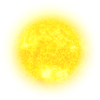
\includegraphics[scale=0.8]{sun}  \\
Меркурий & 
\includegraphics[scale=0.5]{mercury}   \\
Венера & 
\includegraphics[scale=1.2]{venus}   \\
Земля & 
\includegraphics[scale=0.5]{earth}   \\
Марс & 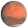
\includegraphics[scale=1.7]{mars}   \\
Юпитер &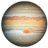
\includegraphics[scale=0.8]{jupiter}    \\
Сатурн & 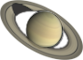
\includegraphics[scale=0.8]{saturn}  \\
Уран & 
\includegraphics[scale=0.8]{uranus}  \\
Нептун & 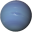
\includegraphics[scale=0.8]{neptune}  \\
\hline
\end{tabular}
%\specialcell{атмосферное \\  давление \\ от земного  } 


\subsection{Орбитальные данные планет}
\begin{tabular}{|p{2.5cm}|p{2.5cm}|p{2cm}|p{2.5cm}|p{2.5cm}|} \hline

\label{table:questions1}
name & ${ orbit_{excenter}}$ & ${orbit_{year}}$ & ${orbit_{speed}}$ &  \\
\hline
Меркурий & 0.206 & 88 & 29.783 &  \\
Венера & 0.0068 & 222.7 & 29.783 &   \\
Земля & 0.017 & 1 год & 29.783 &  \\
Марс & 0.093 & 687 & 29.783 & \\
Юпитер & 0.048 & 4330 & 47.87 &   \\
Сатурн & 0.056 & 29.4 & 9.66 &   \\
Уран & 0.046 & 83.8 & 6.8 &  \\
Нептун & 0.008 & 163.8 & 5.44 &   \\
\hline
& & &  &  ${orbit_{size}}$\\
Меркурий &  &  & & 0.093 \\
Венера &  & &  & 1  \\
Земля &  &  &  & 1 \\
Марс &  &  &  & 1\\
Юпитер &  &  &  & 0.048  \\
Сатурн &  &  &  & 9.55  \\
Уран &  &  &  & 19.2 \\
Нептун &  &  &  & 30.1  \\
\hline
\end{tabular}

\subsection{Физические характеристики планет}
\begin{tabular}{|p{2.5cm}|p{3cm}|p{2cm}|p{3.5cm}|p{1.5cm}|} \hline

\label{table:questions1}
name & ${ mass_{mantissa}}$ & ${mass_{exp}}$ & ${volume_{mantissa}}$ & ${volume_exp}$  \\
\hline
Меркурий & 5.9726 & 24 & 10.8321 & 11 \\
Венера & 5.97 & 24 & 10.8321 & 11  \\
Земля &  5.9726 & 24 &  10.8321 & 11 \\
Марс & 5.9726 & 24 & 10.8321 & 11\\
Юпитер & 1.9 & 30 & 9.2 & 14  \\
Сатурн & 5.69 & 29 & 8.27 & 14  \\
Уран & 8.68 & 28 &  6.8 & 13 \\
Нептун & 1.02 & 29 & 6.25 & 13  \\
\hline
&   &  \specialcell{${Pl_{radius}}$,\\ km} & \specialcell{area,\\ ${ 10^10 km^2}$} & tilt\\
Меркурий &  & 6371 & {$0.05$} & 23.44 \\
Венера &  & 6371 & {$0.05$} & 23.44  \\
Земля &  & 6371 & {$0.05$} & 23.44 \\
Марс &  & 6371 & {$0.05$} & 23.44\\
Юпитер &  & 71492 & 0.5 & 3.13  \\
Сатурн & & 60268 & 6.14 & 25.33  \\
Уран &  & 25559 & 0.8 & 97.86 \\
Нептун &  & 24764 & 0.76 & 28.31  \\
\hline

&  \specialcell{gravity, \\${m/c^2}$} & \specialcell{${space_{speed},\\ km/c^2}$} & {${sidereal_{period}}$,hr} & {temp,${{^\circ} C}$} \\ 
Меркурий & 3.72 & 3.1 & 24 & 435 \\
Венера & 8.87 & 7.36 & 24 & 228  \\
Земля & 9.8 & 7.91 & 24 & -89~---56 \\
Марс & 3.69 & 3.5 & 24 & 216\\
Юпитер & 20.87 & 4.3 & 24 & 127  \\
Сатурн & 7.21 & 7.91 & 10 & 97  \\
Уран &  8.43 & 15,121 & 17 & 53 \\
Нептун & 11,15 & 7.91 & 16 & 72  \\
\hline
&\multicolumn{4}{|c|}{atmo struct, per} \\ \hline
Меркурий & \multicolumn{4}{|c|}{N = 78.08, ${O_2}$ = 20.95, ${H_2}$O vapor = 1, Ag = 0.93, C${O_2}$ = 0.04}   \\ \hline
Венера & \multicolumn{4}{|c|}{N = 78.08, ${O_2}$ = 20.95, ${H_2}$O vapor = 1, Ag = 0.93, C${O_2}$ = 0.04}    \\ \hline
Земля & \multicolumn{4}{|c|}{N = 78.08, ${O_2}$ = 20.95, ${H_2}$O vapor = 1, Ag = 0.93, C${O_2}$ = 0.04}   \\ \hline
Марс & \multicolumn{4}{|c|}{N = 78.08, ${O_2}$ = 20.95, ${H_2}$O vapor = 1, Ag = 0.93, C${O_2}$ = 0.04}  \\ \hline
Юпитер & \multicolumn{4}{|c|}{${H_2}$ = 92, ${He}$ = 8, Ag = 0.10}    \\ \hline
Сатурн & \multicolumn{4}{|c|}{${H_2}$ = 89.6, ${He}$ = 10, Ag = 0.3}    \\ \hline
Уран & \multicolumn{4}{|c|}{{${H_2}$ = 82, ${He}$ = 15, Ag = 2.3}}   \\ \hline
Нептун & \multicolumn{4}{|c|}{{${H_2}$ = 80, ${He}$ = 19, Ag = 1.5}}    \\ \hline
\hline
\end{tabular}
%************************


\end{document}
